\documentclass[12pt]{article}
\usepackage{lingmacros}
\usepackage{tree-dvips}
\usepackage{cmap}
\usepackage[T2A]{fontenc}
\usepackage[utf8]{inputenc}
\usepackage[russian]{babel}
\usepackage{amsmath}
\usepackage{graphicx}


\begin{document}


\section*{Домашная работа по дискретной математике.}

\subsection*{\centering{\underline{TeX Task}}}
\subsection*{Задача о независимом множестве на дереве.
Задача о построении матрицы кратчайших расстояний. 
Метод Флойда-Уоршелла.
}
\subsection*{Author: Gagin Artur, group 172, SE SPbU '25}
\subsection*{Date: Second semester, 2022}

\*
\subsection*{1. Задача о независимом множестве на дереве.}
\underline{Задание}:

Найти максимальное независимое множество вершин на дереве 
(с наибольшим количеством элементов в нем). \\
\underline{Решение}: 

Перед решением быстренько вспомним определение дерева 
в теории графов, а также смысл независимого множества вершин (НМВ далее).

Итак, \textbf{дерево} — это связный ациклический граф. 
Связность в данном случае означает наличие маршрута между любой парой вершин. \\
Ацикличность означает отсутствие циклов. \textbf{Множество вершин графа} называется независимым тогда и только тогда, когда никакие две вершины множества не соединены ребром. 
Теперь, вспомнив эти определения, задача стала совсем ясна.

Попробуем разработать алгоритм, получающий на вход дерево T (с корнем r), который возвращает мощность наибольшего МНВ.

Будем решать задачу, двигаясь по дереву снизу вверх. Сначала будем рассматривать множества, состоящие из одних только листьев, постепенно поднимаясь вверх, увеличивая мощности рассматриваемых множеств.

Заметим, что нам недостаточно иметь значение максимального \\ независимого
 множества вершин в каком-либо поддереве, решая задачу расширением 
 (добавлением выше находящихся узлов), поскольку когда мы добавим новый узел (стоящий выше), нам важно знать,\
 можем ли мы его включить, либо же не можем. Для этого можно рассматривать два независимых множества:
 одно будет включать вершину рассматриваего нами поддерева, а другое не будет. Таким образом, когда мы 
 будем добавлять вершину, рассматривая новую совокупность вершин, более большую по количеству, мы однозначно сможем составить 
 независимые множества вершин уже из большего по количеству вершин дерева.

 Взглянем на пример:

 \begin{figure}[h]
  \begin{minipage}[h]{0.49\linewidth}
  \center{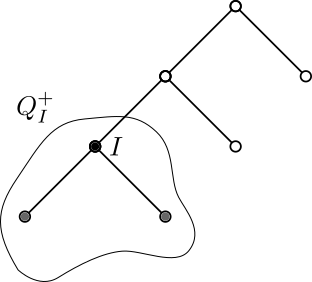
\includegraphics[width=0.5\linewidth]{1} \\ а)}
  \end{minipage}
  \hfill
  \begin{minipage}[h]{0.49\linewidth}
  \center{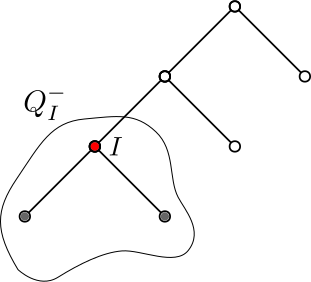
\includegraphics[width=0.5\linewidth]{2} \\ б)}
  \end{minipage}
  \caption{Рисунок 1 и 2.}
  \end{figure}

 Будем обозначать за $Q_{I}^+$ мощность максимального НМВ поддерева, вершина (корень) 
 которого -- узел I, а узлы -- все те, которые находятся глубже вершины I, при этом 
 вершина I обязательно включена в это максимальное НМВ. За $Q_{I}^-$ будем обозначать практически тоже самое,
 но вершина I обязательно не включена в это максимальное НМВ. Теперь, когда мы захотим рассмотреть новое дерево, вершина которого будет являться родителем вершины I, мы однозначно сможем найти мощность МНВ (максимальную ).

 Попытаемся написать рекурсивную формулу, за основу взяв ситуации, когда вершина является листом.

 Очевидно, что если наше множество состоит из одной вершины, то $Q_{I}^+ = 1$ (сама вершина) и $Q_{I}^- = 0$ (здесь стоит отметить, что пустое множество тоже является НМВ). 
 Тогда формулы приобретают следующий вид:
    \begin{equation*}
    Q_{I}^+ =  
     \begin{cases}
       1 &\text{, $I$ является листом}\\
       ... &\text{, $I$ не является листом}
     \end{cases}
    \end{equation*}

    \begin{equation*}
        Q_{I}^- =  
         \begin{cases}
           0 &\text{, $I$ является листом}\\
           ... &\text{, $I$ не является листом}
         \end{cases}
        \end{equation*}

Хорошо, но что насчет ситуаций, когда $I$ не является листом? Попробуем разобраться на примере.

\begin{figure}[h]
  \begin{minipage}[h]{0.49\linewidth}
  \center{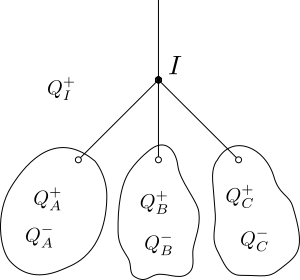
\includegraphics[width=0.5\linewidth]{3} \\ а)}
  \end{minipage}
  \hfill
  \begin{minipage}[h]{0.49\linewidth}
  \center{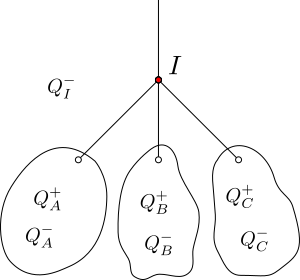
\includegraphics[width=0.5\linewidth]{4} \\ б)}
  \end{minipage}
  \caption{Рисунок 3 и 4.}
  \end{figure}

  $Q_{I}^+$: это максимальное НМВ включает саму вершину $I$, поэтому мы ее считаем. Далее, нам надо взять максимальное МНВ слева (от вершины $A$). Так как вершины не должны быть связаны,
  то это будет $Q_{A}^-$. По такой же логике берем $Q_{B}^-$ и $Q_{C}^-$. Сложив их и прибавив к единице, получим искомую максимальную мощность МНВ поддерева, вершина которого -- $I$.
  
  По похожей логике вычисляется $Q_{I}^-$: здесь мы единичку прибавлять не будем, ведь мы не включаем саму вершину $I$. Также, так как вершина не включена, мы имеем возможность взять как, например, $Q_{A}^+$, так и, например, $Q_{A}^-$. Поскольку мы ищем максимальное МНВ, то будем брать максимум между этими двумя мощностями. 

Итак, завершая данную логику, приходим к выводу, что наши формулы будут выглядеть следующим образом:
\begin{equation*}
  Q_{I}^+ =  
   \begin{cases}
     1 &\text{, $I$ является листом}\\
     1+ \sum_{i \ \in \ child(I)} Q_{i}^- &\text{, $I$ не является листом}
   \end{cases}
  \end{equation*}

  \begin{equation*}
      Q_{I}^- =  
       \begin{cases}
         0 &\text{, $I$ является листом}\\
         \sum_{i \ \in \ child(I)} max\{Q_{i}^+, Q_{i}^-\} &\text{, $I$ не является листом}
       \end{cases}
      \end{equation*}
Дойдя до корня, у нас будет пара чисел: $Q_{R}^+$ и $Q_{R}^-$. Максимальное из них и будет являться ответом на поставленную задачу.

Оценим сложность работы алгоритма: легко заметить, что мы проходим по всем вершинам, при этом ребро обрабатывается один или два раза. 

Таким образом: $O(|V| + |E|)$ (отбросив const).
\bigbreak
Попробуем решить данную задачу на искусственном примере (Рисунок 5) для того, чтобы еще точнее понять, как работает алгоритм, а также для того, чтобы убедиться, что логика, построенная нами,
верна.

\begin{figure}[h]
  \center{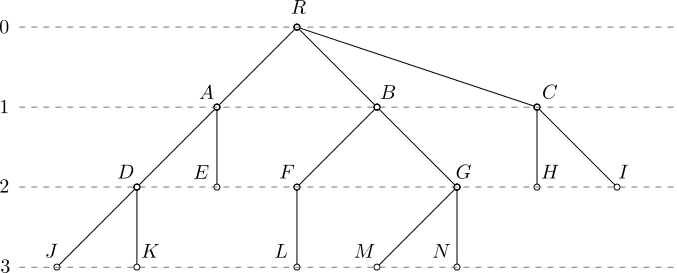
\includegraphics[width=1\linewidth]{5}}
  \caption{Рисунок 5.}
  \label{ris:image}
  \end{figure}

Использовав наивный алгоритм (перебрав все возможные множества), легко понять, что мощность максимального МНВ равна 9. 

Решим пример с помощью наших формул. Начнем с глубины 3:

$Q_{J}^- = 0$, $Q_{J}^+ = 1$;

$Q_{K}^- = 0$, $Q_{K}^+ = 1$;

$Q_{L}^- = 0$, $Q_{L}^+ = 1$;

$Q_{M}^- = 0$, $Q_{M}^+ = 1$;

$Q_{N}^- = 0$, $Q_{N}^+ = 1$;

Глубина 2:

$Q_{D}^- = max\{Q_{J}^- = 0$, $Q_{J}^+ = 1\} + max\{Q_{K}^- = 0$, $Q_{K}^+ = 1\} = 2$, $Q_{D}^+ = 1 + Q_{J}^- + Q_{K}^- = 1 + 0 + 0 = 1 $;

$Q_{E}^- = 0$, $Q_{E}^+ = 1$;

$Q_{F}^- = 1$, $Q_{F}^+ = 1 + 0 = 1$;

$Q_{G}^- = 2$, $Q_{G}^+ = 1$ (аналогично вершине $D$).

$Q_{H}^- = 0$, $Q_{H}^+ = 1$;

$Q_{I}^- = 0$, $Q_{I}^+ = 1$;

Глубина 1:

$Q_{A}^- = max\{Q_{D}^- = 2, Q_{D}^+ = 1\} + max\{Q_{E}^- = 0, Q_{E}^+ = 1\} = 2 + 1 = 3$, $Q_{A}^+ = 1 + Q_{D}^- + Q_{E}^- = 1 + 2 + 0 = 3$;

$Q_{B}^- = max\{Q_{F}^- = 1, Q_{F}^+ = 1\} + max\{Q_{G}^- = 2, Q_{G}^+ = 1\} = 1 + 2 = 3$, $Q_{B}^+ = 1 + Q_{F}^- + Q_{G}^- = 1 + 1 + 2 = 4$;

$Q_{C}^- = 2$, $Q_{C}^+ = 1$;

Глубина 0:

$Q_{R}^- = max\{Q_{A}^- = 3, Q_{A}^+ = 3\} + max\{Q_{B}^- = 3, Q_{B}^+ = 4\} + max\{Q_{C}^- = 2, Q_{C}^+ = 1\} = 3 + 4 + 2 = 9$, $Q_{R}^+ = 1 + Q_{A}^- + Q_{B}^- + Q_{C}^- = 1 + 3 + 3 + 2 = 9$.

Ответом будет служить максимальное из чисел, то есть 9. Что мы и получили, сославшись на наивное решение. 

Таким образом можем заключить, что проблема решена. Мы составили рекурсивную формулу, которая решает поставленную нами задачу.


\subsection*{2. Задача о построении матрицы кратчайших расстояний. Метод Флойда-Уоршелла.}
\underline{Задание}:

Найти кратчайшие пути для любой пары вершин во взвешенном ориентированном графе (тем самым построив матрицу), воспользовавшись для данного задания методом Флойда-Уоршелла. \\
\underline{Решение}: 

Перед решением предлагаем вспомнить, что такое взвешенный граф. \textbf{Взвешенным графом} называется граф, каждому ребру которого поставлено в соответствие некое значение (вес ребра).
\textbf{Кратчайшее расстояние между узлами в графе} -- такое расстояние, при котором сумма весов составляющих его ребер минимальна.
\textbf{Алгоритм Флойда — Уоршелла} -- это алгоритм поиска кратчайших путей во взвешенном (ориентированном в том числе) графе с положительным или отрицательным весом ребер (но без отрицательных циклов).

Рассмотрим идею данного алгоритма: пусть у нас есть две вершины $i$ и $k$, а также 
расстояние из одной вершины в другую (существует возможность попасть из
 первой вершины в последнюю). Рассмотрим также и вспомогательную вершину $j$, 
 для которой выполняется следующее условие: из вершины $i$ можно попасть в 
 вершину $j$, из вершины $j$ можно попасть в вершину $k$. При этом расстояния
  из вершины $i$ в вершину $j$ и из вершины $j$ в вершину $k$ не должны равняться
   бесконечности. Обозначим эти расстояния $d_{ij}$ и $d_{jk}$. Рассмотрим сумму
    этих расстояний. Если $d_{ij} + d{jk} < d_{ik}$ (наше первоначальное
     расстояние), то мы заменяем это первоначальное расстояние в нашей матрице 
     на полученную сумму.

Попробуем реализовать данный алгоритм на языке программирования C\#. Данную идею алгоритма можно реализовать следующим образом: 

\begin{center}
d[i, j] = Math.Min(d[i, j], d[i, k] + d[k, j]); 
\end{center}
Стоит отметить, что если в графе не существует расстояния из одной вершины в другую, то такое расстояние мы будем отмечать бесконечностью. Расстояние из вершины в себя отмечаем нулем.

Рассмотрим идею на следующем примере:
\\
\\
\\
\begin{minipage}[h]{0.59\linewidth}
  \center{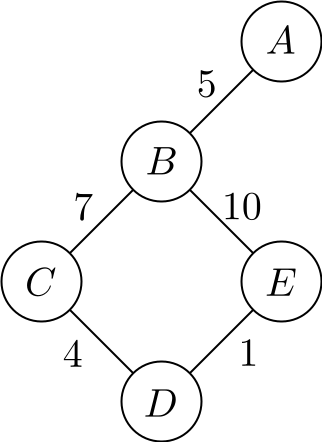
\includegraphics[width=0.5\linewidth]{6} \\ Рисунок 6.}
\end{minipage}
\\
\\
\\
На первом шаге мы просто получаем наш граф на вход. Матрица смежности будет выглядеть следующим образом (вершины в графе пронумерованы):
\begin{center}
$\begin{bmatrix}
   & (1)& (2)& (3)& (4)& (5)\\
  (1)& 0& 5& \infty& \infty& \infty\\
  (2)& 5& 0& 7& \infty& 10\\
  (3)& \infty& 7& 0& 4& \infty\\
  (4)& \infty& \infty& 4& 0& 1\\
  (5)& \infty& 10& \infty& 1& 0 
\end{bmatrix}$
\end{center}
То есть, на ней отображены расстояния от вершин к близлежащим им вершинам. Стоит отметить, что в данном примере
 мы рассматриваем неориентированный граф, поэтому матрица, 
 подаваемая на вход, получилась симметричная. Очевидно, что все
  следующие действия, проделываемые нами в этом примере, будут
   работать и для ориентированного графа, просто он перестанет быть симметричным.
   
Далее, мы разобьем наш алгоритм на шаги, в каждом из которых мы будем рассматривать по вершине. То есть, всего шагов будет столько, сколько вершин в нашем графе. 
Нам необходимо рассмотреть функцию, которая возвращает кратчайший возможный путь от $i$ до $j$ с  использованием вершин только из множества $\{1,2,\ldots ,k\}$ в качестве промежуточных точек на этом пути, где $k$ -- номер нашего шага. 
Перед $k$-тым шагом мы будем считать, $d_{ij}$ -- длина кратчайшего пути из вершины $i$ в вершину $j$.

Рассмотрим $k = 1$.
Идейно, мы рассматриваем вершину с этим номером как дополнительную вершину. Берем каждую пару вершин $i$ и $j$, а затем смотрим, может ли эта вершина $k$ повлиять на расстояние между этими вершинами, можно ли, пройдя только через вершины $\{1,2,\ldots ,k\}$, как дополнительные, попасть из одной в другую за меньшее расстояние. Из рисунка очевидно, что вершина $A (1)$ никаким образом не способна повлиять на расстояния между какими-либо парами вершин. Таким образом, матрица после первого шага сохраняется (остается прежней).

Рассмотрим $k = 2$.
Теперь смотрим, можем ли мы с помощью второй вершины найти новые кратчайшие пути для пар вершин. Очевидно, что это можно сделать. Например, из вершины $A (1)$ в вершину $C (3)$ можно попасть с помощью второй вершины: $(1)\rightarrow(3) = (1)\rightarrow(2) + (2)\rightarrow(3)$.
Для пары $1$ и $4$ это невозможно сделать, поскольку, хоть и первой вершины во вторую у нас существует путь, из второй вершины в четвертую пути нет (бесконечность).
Таким же образом рассматриваем оставшиеся пары. То есть, пути из $i$ в $k$, из $k$ в $j$. Если их сумма меньше существующего расстояния из $i$ в $j$, то записываем в матрицу значение суммы.
Результат после второго шага выглядит следующим образом:
\begin{center}
  $\begin{bmatrix}
     & (1)& (2)& (3)& (4)& (5)\\
    (1)& 0& 5& 12& \infty& 15\\
    (2)& 5& 0& 7& \infty& 10\\
    (3)& 12& 7& 0& 4& 17\\
    (4)& \infty& \infty& 4& 0& 1\\
    (5)& 15& 10& 17& 1& 0 
  \end{bmatrix}$
  \end{center}

Рассмотрим $k = 3$.
Результат после третьего шага выглядит следующим образом:
\begin{center}
  $\begin{bmatrix}
     & (1)& (2)& (3)& (4)& (5)\\
    (1)& 0& 5& 12& 16& 15\\
    (2)& 5& 0& 7& 11& 10\\
    (3)& 12& 7& 0& 4& 17\\
    (4)& 16& 11& 4& 0& 1\\
    (5)& 15& 10& 17& 1& 0 
  \end{bmatrix}$
  \end{center}

  Рассмотрим $k = 4$.
  Результат после четвертого шага выглядит следующим образом:
  \begin{center}
    $\begin{bmatrix}
       & (1)& (2)& (3)& (4)& (5)\\
      (1)& 0& 5& 12& 16& 15\\
      (2)& 5& 0& 7& 11& 10\\
      (3)& 12& 7& 0& 4& 5\\
      (4)& 16& 11& 4& 0& 1\\
      (5)& 15& 10& 5& 1& 0 
    \end{bmatrix}$
    \end{center}

    Рассмотрим $k = 5$.
    Результат после этого шага выглядит аналогично матрице выше.

\*
Так что насчет реализации данного алгоритма? Все достаточно просто:

\begin{verbatim}
  using System;
  namespace FloydAlgorithm
  {
      class Program
      {
          static void Main(string[] args)
          {
              Console.WriteLine("Введите количество вершин в графе:");
              var n = Int32.Parse(Console.ReadLine());
              var matrix = new double[n, n];
              for (var i = 0; i < n; i++)
              {
                  for (var j = 0; j < n; j++)
                  {
                      Console.WriteLine(
                          $"Введите расстояние между вершинами {i + 1} и {j + 1}. Если они соединены ребром, то введите расстояние. Если они НЕ соединены ребром, то введите NO. Если вершина одна и та же, то введите 0:");
                      var answer = Console.ReadLine();
                      if (double.TryParse(answer, out var doubleAnswer))
                      {
                          matrix[i, j] = doubleAnswer;
                      }
                      else
                      {
                          matrix[i, j] = double.PositiveInfinity;
                      }
                  }
              }
              Console.WriteLine("Ответ:");
              for (var k = 0; k < n; k++)
              {
                  for (var i = 0; i < n; i++)
                  {
                      for (var j = 0; j < n; j++)
                      {
                          matrix[i, j] = Math.Min(matrix[i, j], matrix[i, k] + matrix[k, j]);
                      }
                  }
              }
  
              for (var i = 0; i < n; i++)
              {
                  for (var j = 0; j < n; j++)
                  {
                      Console.Write($"{matrix[i, j]} ");
                  }
                  Console.WriteLine();
              }
          }
      }
  }
  \end{verbatim}

Таким образом, сложность работы данного алгоритма составляет $O(N^3)$, где $N$ -- количество вершин в графе. Наша задача решена.
\end{document}